% Created by tikzDevice version 0.12.3.1 on 2023-02-11 15:38:51
% !TEX encoding = UTF-8 Unicode
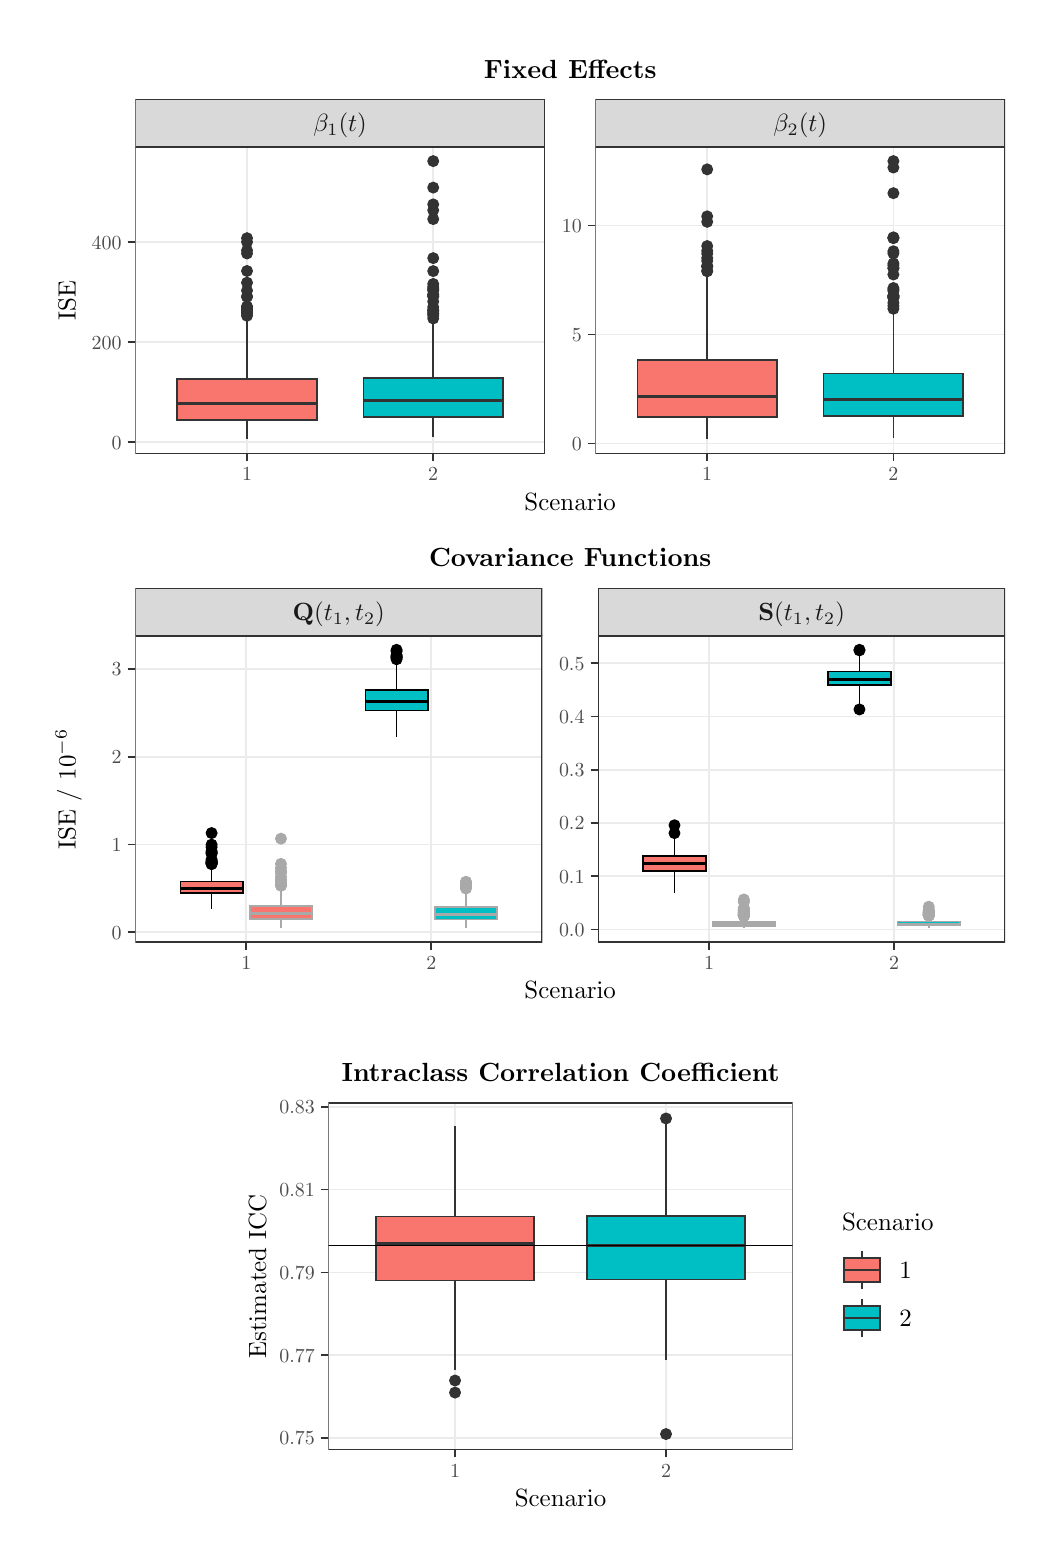
\begin{tikzpicture}[x=1pt,y=1pt]
\definecolor{fillColor}{RGB}{255,255,255}
\path[use as bounding box,fill=fillColor,fill opacity=0.00] (0,0) rectangle (364.19,546.29);
\begin{scope}
\path[clip] (  0.00,182.10) rectangle (364.19,546.29);
\definecolor{drawColor}{RGB}{255,255,255}
\definecolor{fillColor}{RGB}{255,255,255}

\path[draw=drawColor,line width= 0.6pt,line join=round,line cap=round,fill=fillColor] (  0.00,182.10) rectangle (364.19,546.29);
\end{scope}
\begin{scope}
\path[clip] (  5.50,364.19) rectangle (358.69,540.79);
\definecolor{drawColor}{RGB}{255,255,255}
\definecolor{fillColor}{RGB}{255,255,255}

\path[draw=drawColor,line width= 0.6pt,line join=round,line cap=round,fill=fillColor] (  5.50,364.19) rectangle (358.69,540.79);
\end{scope}
\begin{scope}
\path[clip] ( 38.89,392.46) rectangle (186.91,503.10);
\definecolor{fillColor}{RGB}{255,255,255}

\path[fill=fillColor] ( 38.89,392.46) rectangle (186.91,503.10);
\definecolor{drawColor}{gray}{0.92}

\path[draw=drawColor,line width= 0.6pt,line join=round] ( 38.89,396.46) --
	(186.91,396.46);

\path[draw=drawColor,line width= 0.6pt,line join=round] ( 38.89,432.62) --
	(186.91,432.62);

\path[draw=drawColor,line width= 0.6pt,line join=round] ( 38.89,468.77) --
	(186.91,468.77);

\path[draw=drawColor,line width= 0.6pt,line join=round] ( 79.26,392.46) --
	( 79.26,503.10);

\path[draw=drawColor,line width= 0.6pt,line join=round] (146.54,392.46) --
	(146.54,503.10);
\definecolor{drawColor}{gray}{0.20}
\definecolor{fillColor}{gray}{0.20}

\path[draw=drawColor,line width= 0.4pt,line join=round,line cap=round,fill=fillColor] ( 79.26,442.19) circle (  1.96);

\path[draw=drawColor,line width= 0.4pt,line join=round,line cap=round,fill=fillColor] ( 79.26,443.80) circle (  1.96);

\path[draw=drawColor,line width= 0.4pt,line join=round,line cap=round,fill=fillColor] ( 79.26,445.22) circle (  1.96);

\path[draw=drawColor,line width= 0.4pt,line join=round,line cap=round,fill=fillColor] ( 79.26,443.83) circle (  1.96);

\path[draw=drawColor,line width= 0.4pt,line join=round,line cap=round,fill=fillColor] ( 79.26,445.11) circle (  1.96);

\path[draw=drawColor,line width= 0.4pt,line join=round,line cap=round,fill=fillColor] ( 79.26,443.83) circle (  1.96);

\path[draw=drawColor,line width= 0.4pt,line join=round,line cap=round,fill=fillColor] ( 79.26,451.30) circle (  1.96);

\path[draw=drawColor,line width= 0.4pt,line join=round,line cap=round,fill=fillColor] ( 79.26,465.80) circle (  1.96);

\path[draw=drawColor,line width= 0.4pt,line join=round,line cap=round,fill=fillColor] ( 79.26,443.37) circle (  1.96);

\path[draw=drawColor,line width= 0.4pt,line join=round,line cap=round,fill=fillColor] ( 79.26,443.90) circle (  1.96);

\path[draw=drawColor,line width= 0.4pt,line join=round,line cap=round,fill=fillColor] ( 79.26,444.15) circle (  1.96);

\path[draw=drawColor,line width= 0.4pt,line join=round,line cap=round,fill=fillColor] ( 79.26,464.69) circle (  1.96);

\path[draw=drawColor,line width= 0.4pt,line join=round,line cap=round,fill=fillColor] ( 79.26,449.14) circle (  1.96);

\path[draw=drawColor,line width= 0.4pt,line join=round,line cap=round,fill=fillColor] ( 79.26,454.14) circle (  1.96);

\path[draw=drawColor,line width= 0.4pt,line join=round,line cap=round,fill=fillColor] ( 79.26,468.83) circle (  1.96);

\path[draw=drawColor,line width= 0.4pt,line join=round,line cap=round,fill=fillColor] ( 79.26,458.37) circle (  1.96);

\path[draw=drawColor,line width= 0.4pt,line join=round,line cap=round,fill=fillColor] ( 79.26,443.87) circle (  1.96);

\path[draw=drawColor,line width= 0.4pt,line join=round,line cap=round,fill=fillColor] ( 79.26,470.22) circle (  1.96);

\path[draw=drawColor,line width= 0.4pt,line join=round,line cap=round,fill=fillColor] ( 79.26,449.05) circle (  1.96);

\path[draw=drawColor,line width= 0.4pt,line join=round,line cap=round,fill=fillColor] ( 79.26,443.10) circle (  1.96);

\path[draw=drawColor,line width= 0.4pt,line join=round,line cap=round,fill=fillColor] ( 79.26,443.19) circle (  1.96);

\path[draw=drawColor,line width= 0.4pt,line join=round,line cap=round,fill=fillColor] ( 79.26,445.52) circle (  1.96);

\path[draw=drawColor,line width= 0.4pt,line join=round,line cap=round,fill=fillColor] ( 79.26,445.24) circle (  1.96);

\path[draw=drawColor,line width= 0.6pt,line join=round] ( 79.26,419.23) -- ( 79.26,441.33);

\path[draw=drawColor,line width= 0.6pt,line join=round] ( 79.26,404.49) -- ( 79.26,397.49);
\definecolor{fillColor}{RGB}{248,118,109}

\path[draw=drawColor,line width= 0.6pt,fill=fillColor] ( 54.03,419.23) --
	( 54.03,404.49) --
	(104.49,404.49) --
	(104.49,419.23) --
	( 54.03,419.23) --
	cycle;

\path[draw=drawColor,line width= 1.1pt] ( 54.03,410.34) -- (104.49,410.34);
\definecolor{fillColor}{gray}{0.20}

\path[draw=drawColor,line width= 0.4pt,line join=round,line cap=round,fill=fillColor] (146.54,458.32) circle (  1.96);

\path[draw=drawColor,line width= 0.4pt,line join=round,line cap=round,fill=fillColor] (146.54,447.33) circle (  1.96);

\path[draw=drawColor,line width= 0.4pt,line join=round,line cap=round,fill=fillColor] (146.54,488.50) circle (  1.96);

\path[draw=drawColor,line width= 0.4pt,line join=round,line cap=round,fill=fillColor] (146.54,480.31) circle (  1.96);

\path[draw=drawColor,line width= 0.4pt,line join=round,line cap=round,fill=fillColor] (146.54,482.43) circle (  1.96);

\path[draw=drawColor,line width= 0.4pt,line join=round,line cap=round,fill=fillColor] (146.54,449.18) circle (  1.96);

\path[draw=drawColor,line width= 0.4pt,line join=round,line cap=round,fill=fillColor] (146.54,443.00) circle (  1.96);

\path[draw=drawColor,line width= 0.4pt,line join=round,line cap=round,fill=fillColor] (146.54,453.68) circle (  1.96);

\path[draw=drawColor,line width= 0.4pt,line join=round,line cap=round,fill=fillColor] (146.54,443.79) circle (  1.96);

\path[draw=drawColor,line width= 0.4pt,line join=round,line cap=round,fill=fillColor] (146.54,441.21) circle (  1.96);

\path[draw=drawColor,line width= 0.4pt,line join=round,line cap=round,fill=fillColor] (146.54,444.22) circle (  1.96);

\path[draw=drawColor,line width= 0.4pt,line join=round,line cap=round,fill=fillColor] (146.54,442.98) circle (  1.96);

\path[draw=drawColor,line width= 0.4pt,line join=round,line cap=round,fill=fillColor] (146.54,477.12) circle (  1.96);

\path[draw=drawColor,line width= 0.4pt,line join=round,line cap=round,fill=fillColor] (146.54,451.29) circle (  1.96);

\path[draw=drawColor,line width= 0.4pt,line join=round,line cap=round,fill=fillColor] (146.54,449.90) circle (  1.96);

\path[draw=drawColor,line width= 0.4pt,line join=round,line cap=round,fill=fillColor] (146.54,442.27) circle (  1.96);

\path[draw=drawColor,line width= 0.4pt,line join=round,line cap=round,fill=fillColor] (146.54,445.32) circle (  1.96);

\path[draw=drawColor,line width= 0.4pt,line join=round,line cap=round,fill=fillColor] (146.54,463.01) circle (  1.96);

\path[draw=drawColor,line width= 0.4pt,line join=round,line cap=round,fill=fillColor] (146.54,452.63) circle (  1.96);

\path[draw=drawColor,line width= 0.4pt,line join=round,line cap=round,fill=fillColor] (146.54,444.23) circle (  1.96);

\path[draw=drawColor,line width= 0.4pt,line join=round,line cap=round,fill=fillColor] (146.54,452.12) circle (  1.96);

\path[draw=drawColor,line width= 0.4pt,line join=round,line cap=round,fill=fillColor] (146.54,449.22) circle (  1.96);

\path[draw=drawColor,line width= 0.4pt,line join=round,line cap=round,fill=fillColor] (146.54,451.60) circle (  1.96);

\path[draw=drawColor,line width= 0.4pt,line join=round,line cap=round,fill=fillColor] (146.54,498.07) circle (  1.96);

\path[draw=drawColor,line width= 0.4pt,line join=round,line cap=round,fill=fillColor] (146.54,449.72) circle (  1.96);

\path[draw=drawColor,line width= 0.6pt,line join=round] (146.54,419.71) -- (146.54,440.16);

\path[draw=drawColor,line width= 0.6pt,line join=round] (146.54,405.55) -- (146.54,398.55);
\definecolor{fillColor}{RGB}{0,191,196}

\path[draw=drawColor,line width= 0.6pt,fill=fillColor] (121.31,419.71) --
	(121.31,405.55) --
	(171.77,405.55) --
	(171.77,419.71) --
	(121.31,419.71) --
	cycle;

\path[draw=drawColor,line width= 1.1pt] (121.31,411.51) -- (171.77,411.51);

\path[draw=drawColor,line width= 0.6pt,line join=round,line cap=round] ( 38.89,392.46) rectangle (186.91,503.10);
\end{scope}
\begin{scope}
\path[clip] (205.18,392.46) rectangle (353.19,503.10);
\definecolor{fillColor}{RGB}{255,255,255}

\path[fill=fillColor] (205.18,392.46) rectangle (353.19,503.10);
\definecolor{drawColor}{gray}{0.92}

\path[draw=drawColor,line width= 0.6pt,line join=round] (205.18,396.08) --
	(353.19,396.08);

\path[draw=drawColor,line width= 0.6pt,line join=round] (205.18,435.43) --
	(353.19,435.43);

\path[draw=drawColor,line width= 0.6pt,line join=round] (205.18,474.78) --
	(353.19,474.78);

\path[draw=drawColor,line width= 0.6pt,line join=round] (245.54,392.46) --
	(245.54,503.10);

\path[draw=drawColor,line width= 0.6pt,line join=round] (312.83,392.46) --
	(312.83,503.10);
\definecolor{drawColor}{gray}{0.20}
\definecolor{fillColor}{gray}{0.20}

\path[draw=drawColor,line width= 0.4pt,line join=round,line cap=round,fill=fillColor] (245.54,460.20) circle (  1.96);

\path[draw=drawColor,line width= 0.4pt,line join=round,line cap=round,fill=fillColor] (245.54,464.62) circle (  1.96);

\path[draw=drawColor,line width= 0.4pt,line join=round,line cap=round,fill=fillColor] (245.54,459.94) circle (  1.96);

\path[draw=drawColor,line width= 0.4pt,line join=round,line cap=round,fill=fillColor] (245.54,463.05) circle (  1.96);

\path[draw=drawColor,line width= 0.4pt,line join=round,line cap=round,fill=fillColor] (245.54,465.68) circle (  1.96);

\path[draw=drawColor,line width= 0.4pt,line join=round,line cap=round,fill=fillColor] (245.54,476.13) circle (  1.96);

\path[draw=drawColor,line width= 0.4pt,line join=round,line cap=round,fill=fillColor] (245.54,458.43) circle (  1.96);

\path[draw=drawColor,line width= 0.4pt,line join=round,line cap=round,fill=fillColor] (245.54,478.10) circle (  1.96);

\path[draw=drawColor,line width= 0.4pt,line join=round,line cap=round,fill=fillColor] (245.54,458.26) circle (  1.96);

\path[draw=drawColor,line width= 0.4pt,line join=round,line cap=round,fill=fillColor] (245.54,467.37) circle (  1.96);

\path[draw=drawColor,line width= 0.4pt,line join=round,line cap=round,fill=fillColor] (245.54,462.01) circle (  1.96);

\path[draw=drawColor,line width= 0.4pt,line join=round,line cap=round,fill=fillColor] (245.54,460.06) circle (  1.96);

\path[draw=drawColor,line width= 0.4pt,line join=round,line cap=round,fill=fillColor] (245.54,495.08) circle (  1.96);

\path[draw=drawColor,line width= 0.6pt,line join=round] (245.54,426.31) -- (245.54,457.22);

\path[draw=drawColor,line width= 0.6pt,line join=round] (245.54,405.67) -- (245.54,397.49);
\definecolor{fillColor}{RGB}{248,118,109}

\path[draw=drawColor,line width= 0.6pt,fill=fillColor] (220.31,426.31) --
	(220.31,405.67) --
	(270.77,405.67) --
	(270.77,426.31) --
	(220.31,426.31) --
	cycle;

\path[draw=drawColor,line width= 1.1pt] (220.31,413.15) -- (270.77,413.15);
\definecolor{fillColor}{gray}{0.20}

\path[draw=drawColor,line width= 0.4pt,line join=round,line cap=round,fill=fillColor] (312.83,470.52) circle (  1.96);

\path[draw=drawColor,line width= 0.4pt,line join=round,line cap=round,fill=fillColor] (312.83,465.50) circle (  1.96);

\path[draw=drawColor,line width= 0.4pt,line join=round,line cap=round,fill=fillColor] (312.83,498.07) circle (  1.96);

\path[draw=drawColor,line width= 0.4pt,line join=round,line cap=round,fill=fillColor] (312.83,449.24) circle (  1.96);

\path[draw=drawColor,line width= 0.4pt,line join=round,line cap=round,fill=fillColor] (312.83,448.67) circle (  1.96);

\path[draw=drawColor,line width= 0.4pt,line join=round,line cap=round,fill=fillColor] (312.83,460.44) circle (  1.96);

\path[draw=drawColor,line width= 0.4pt,line join=round,line cap=round,fill=fillColor] (312.83,495.74) circle (  1.96);

\path[draw=drawColor,line width= 0.4pt,line join=round,line cap=round,fill=fillColor] (312.83,464.71) circle (  1.96);

\path[draw=drawColor,line width= 0.4pt,line join=round,line cap=round,fill=fillColor] (312.83,444.71) circle (  1.96);

\path[draw=drawColor,line width= 0.4pt,line join=round,line cap=round,fill=fillColor] (312.83,457.09) circle (  1.96);

\path[draw=drawColor,line width= 0.4pt,line join=round,line cap=round,fill=fillColor] (312.83,486.48) circle (  1.96);

\path[draw=drawColor,line width= 0.4pt,line join=round,line cap=round,fill=fillColor] (312.83,451.68) circle (  1.96);

\path[draw=drawColor,line width= 0.4pt,line join=round,line cap=round,fill=fillColor] (312.83,449.29) circle (  1.96);

\path[draw=drawColor,line width= 0.4pt,line join=round,line cap=round,fill=fillColor] (312.83,448.69) circle (  1.96);

\path[draw=drawColor,line width= 0.4pt,line join=round,line cap=round,fill=fillColor] (312.83,452.21) circle (  1.96);

\path[draw=drawColor,line width= 0.4pt,line join=round,line cap=round,fill=fillColor] (312.83,470.27) circle (  1.96);

\path[draw=drawColor,line width= 0.4pt,line join=round,line cap=round,fill=fillColor] (312.83,461.11) circle (  1.96);

\path[draw=drawColor,line width= 0.4pt,line join=round,line cap=round,fill=fillColor] (312.83,451.15) circle (  1.96);

\path[draw=drawColor,line width= 0.4pt,line join=round,line cap=round,fill=fillColor] (312.83,459.42) circle (  1.96);

\path[draw=drawColor,line width= 0.4pt,line join=round,line cap=round,fill=fillColor] (312.83,445.77) circle (  1.96);

\path[draw=drawColor,line width= 0.4pt,line join=round,line cap=round,fill=fillColor] (312.83,449.29) circle (  1.96);

\path[draw=drawColor,line width= 0.4pt,line join=round,line cap=round,fill=fillColor] (312.83,459.39) circle (  1.96);

\path[draw=drawColor,line width= 0.4pt,line join=round,line cap=round,fill=fillColor] (312.83,449.48) circle (  1.96);

\path[draw=drawColor,line width= 0.4pt,line join=round,line cap=round,fill=fillColor] (312.83,470.27) circle (  1.96);

\path[draw=drawColor,line width= 0.4pt,line join=round,line cap=round,fill=fillColor] (312.83,446.86) circle (  1.96);

\path[draw=drawColor,line width= 0.6pt,line join=round] (312.83,421.38) -- (312.83,444.40);

\path[draw=drawColor,line width= 0.6pt,line join=round] (312.83,405.89) -- (312.83,398.17);
\definecolor{fillColor}{RGB}{0,191,196}

\path[draw=drawColor,line width= 0.6pt,fill=fillColor] (287.60,421.38) --
	(287.60,405.89) --
	(338.06,405.89) --
	(338.06,421.38) --
	(287.60,421.38) --
	cycle;

\path[draw=drawColor,line width= 1.1pt] (287.60,411.83) -- (338.06,411.83);

\path[draw=drawColor,line width= 0.6pt,line join=round,line cap=round] (205.18,392.46) rectangle (353.19,503.10);
\end{scope}
\begin{scope}
\path[clip] (  0.00,  0.00) rectangle (364.19,546.29);
\definecolor{drawColor}{gray}{0.30}

\node[text=drawColor,anchor=base east,inner sep=0pt, outer sep=0pt, scale=  0.72] at (200.23,393.60) {0};

\node[text=drawColor,anchor=base east,inner sep=0pt, outer sep=0pt, scale=  0.72] at (200.23,432.95) {5};

\node[text=drawColor,anchor=base east,inner sep=0pt, outer sep=0pt, scale=  0.72] at (200.23,472.30) {10};
\end{scope}
\begin{scope}
\path[clip] (  0.00,  0.00) rectangle (364.19,546.29);
\definecolor{drawColor}{gray}{0.20}

\path[draw=drawColor,line width= 0.6pt,line join=round] (202.43,396.08) --
	(205.18,396.08);

\path[draw=drawColor,line width= 0.6pt,line join=round] (202.43,435.43) --
	(205.18,435.43);

\path[draw=drawColor,line width= 0.6pt,line join=round] (202.43,474.78) --
	(205.18,474.78);
\end{scope}
\begin{scope}
\path[clip] ( 38.89,503.10) rectangle (186.91,520.38);
\definecolor{drawColor}{gray}{0.20}
\definecolor{fillColor}{gray}{0.85}

\path[draw=drawColor,line width= 0.6pt,line join=round,line cap=round,fill=fillColor] ( 38.89,503.10) rectangle (186.91,520.38);
\definecolor{drawColor}{gray}{0.10}

\node[text=drawColor,anchor=base,inner sep=0pt, outer sep=0pt, scale=  0.90] at (112.90,508.64) {$\beta_1 (t)$};
\end{scope}
\begin{scope}
\path[clip] (205.18,503.10) rectangle (353.19,520.38);
\definecolor{drawColor}{gray}{0.20}
\definecolor{fillColor}{gray}{0.85}

\path[draw=drawColor,line width= 0.6pt,line join=round,line cap=round,fill=fillColor] (205.18,503.10) rectangle (353.19,520.38);
\definecolor{drawColor}{gray}{0.10}

\node[text=drawColor,anchor=base,inner sep=0pt, outer sep=0pt, scale=  0.90] at (279.19,508.64) {$\beta_2 (t)$};
\end{scope}
\begin{scope}
\path[clip] (  0.00,  0.00) rectangle (364.19,546.29);
\definecolor{drawColor}{gray}{0.20}

\path[draw=drawColor,line width= 0.6pt,line join=round] ( 79.26,389.71) --
	( 79.26,392.46);

\path[draw=drawColor,line width= 0.6pt,line join=round] (146.54,389.71) --
	(146.54,392.46);
\end{scope}
\begin{scope}
\path[clip] (  0.00,  0.00) rectangle (364.19,546.29);
\definecolor{drawColor}{gray}{0.30}

\node[text=drawColor,anchor=base,inner sep=0pt, outer sep=0pt, scale=  0.72] at ( 79.26,382.55) {1};

\node[text=drawColor,anchor=base,inner sep=0pt, outer sep=0pt, scale=  0.72] at (146.54,382.55) {2};
\end{scope}
\begin{scope}
\path[clip] (  0.00,  0.00) rectangle (364.19,546.29);
\definecolor{drawColor}{gray}{0.20}

\path[draw=drawColor,line width= 0.6pt,line join=round] (245.54,389.71) --
	(245.54,392.46);

\path[draw=drawColor,line width= 0.6pt,line join=round] (312.83,389.71) --
	(312.83,392.46);
\end{scope}
\begin{scope}
\path[clip] (  0.00,  0.00) rectangle (364.19,546.29);
\definecolor{drawColor}{gray}{0.30}

\node[text=drawColor,anchor=base,inner sep=0pt, outer sep=0pt, scale=  0.72] at (245.54,382.55) {1};

\node[text=drawColor,anchor=base,inner sep=0pt, outer sep=0pt, scale=  0.72] at (312.83,382.55) {2};
\end{scope}
\begin{scope}
\path[clip] (  0.00,  0.00) rectangle (364.19,546.29);
\definecolor{drawColor}{gray}{0.30}

\node[text=drawColor,anchor=base east,inner sep=0pt, outer sep=0pt, scale=  0.72] at ( 33.94,393.98) {0};

\node[text=drawColor,anchor=base east,inner sep=0pt, outer sep=0pt, scale=  0.72] at ( 33.94,430.14) {200};

\node[text=drawColor,anchor=base east,inner sep=0pt, outer sep=0pt, scale=  0.72] at ( 33.94,466.29) {400};
\end{scope}
\begin{scope}
\path[clip] (  0.00,  0.00) rectangle (364.19,546.29);
\definecolor{drawColor}{gray}{0.20}

\path[draw=drawColor,line width= 0.6pt,line join=round] ( 36.14,396.46) --
	( 38.89,396.46);

\path[draw=drawColor,line width= 0.6pt,line join=round] ( 36.14,432.62) --
	( 38.89,432.62);

\path[draw=drawColor,line width= 0.6pt,line join=round] ( 36.14,468.77) --
	( 38.89,468.77);
\end{scope}
\begin{scope}
\path[clip] (  0.00,  0.00) rectangle (364.19,546.29);
\definecolor{drawColor}{RGB}{0,0,0}

\node[text=drawColor,anchor=base,inner sep=0pt, outer sep=0pt, scale=  0.90] at (196.04,371.97) {Scenario};
\end{scope}
\begin{scope}
\path[clip] (  0.00,  0.00) rectangle (364.19,546.29);
\definecolor{drawColor}{RGB}{0,0,0}

\node[text=drawColor,rotate= 90.00,anchor=base,inner sep=0pt, outer sep=0pt, scale=  0.90] at ( 17.34,447.78) {ISE};
\end{scope}
\begin{scope}
\path[clip] (  0.00,  0.00) rectangle (364.19,546.29);
\definecolor{drawColor}{RGB}{0,0,0}

\node[text=drawColor,anchor=base,inner sep=0pt, outer sep=0pt, scale=  0.95] at (196.04,528.08) {\bfseries Fixed Effects};
\end{scope}
\begin{scope}
\path[clip] (  5.50,187.60) rectangle (358.69,364.19);
\definecolor{drawColor}{RGB}{255,255,255}
\definecolor{fillColor}{RGB}{255,255,255}

\path[draw=drawColor,line width= 0.6pt,line join=round,line cap=round,fill=fillColor] (  5.50,187.60) rectangle (358.69,364.19);
\end{scope}
\begin{scope}
\path[clip] ( 38.89,215.86) rectangle (185.94,326.51);
\definecolor{fillColor}{RGB}{255,255,255}

\path[fill=fillColor] ( 38.89,215.86) rectangle (185.94,326.51);
\definecolor{drawColor}{gray}{0.92}

\path[draw=drawColor,line width= 0.6pt,line join=round] ( 38.89,219.39) --
	(185.94,219.39);

\path[draw=drawColor,line width= 0.6pt,line join=round] ( 38.89,251.10) --
	(185.94,251.10);

\path[draw=drawColor,line width= 0.6pt,line join=round] ( 38.89,282.80) --
	(185.94,282.80);

\path[draw=drawColor,line width= 0.6pt,line join=round] ( 38.89,314.51) --
	(185.94,314.51);

\path[draw=drawColor,line width= 0.6pt,line join=round] ( 79.00,215.86) --
	( 79.00,326.51);

\path[draw=drawColor,line width= 0.6pt,line join=round] (145.83,215.86) --
	(145.83,326.51);
\definecolor{drawColor}{RGB}{0,0,0}
\definecolor{fillColor}{RGB}{0,0,0}

\path[draw=drawColor,line width= 0.4pt,line join=round,line cap=round,fill=fillColor] ( 66.46,245.27) circle (  1.96);

\path[draw=drawColor,line width= 0.4pt,line join=round,line cap=round,fill=fillColor] ( 66.46,250.17) circle (  1.96);

\path[draw=drawColor,line width= 0.4pt,line join=round,line cap=round,fill=fillColor] ( 66.46,248.74) circle (  1.96);

\path[draw=drawColor,line width= 0.4pt,line join=round,line cap=round,fill=fillColor] ( 66.46,244.40) circle (  1.96);

\path[draw=drawColor,line width= 0.4pt,line join=round,line cap=round,fill=fillColor] ( 66.46,244.84) circle (  1.96);

\path[draw=drawColor,line width= 0.4pt,line join=round,line cap=round,fill=fillColor] ( 66.46,245.74) circle (  1.96);

\path[draw=drawColor,line width= 0.4pt,line join=round,line cap=round,fill=fillColor] ( 66.46,244.02) circle (  1.96);

\path[draw=drawColor,line width= 0.4pt,line join=round,line cap=round,fill=fillColor] ( 66.46,255.26) circle (  1.96);

\path[draw=drawColor,line width= 0.4pt,line join=round,line cap=round,fill=fillColor] ( 66.46,247.99) circle (  1.96);

\path[draw=drawColor,line width= 0.4pt,line join=round,line cap=round,fill=fillColor] ( 66.46,244.81) circle (  1.96);

\path[draw=drawColor,line width= 0.4pt,line join=round,line cap=round,fill=fillColor] ( 66.46,248.31) circle (  1.96);

\path[draw=drawColor,line width= 0.4pt,line join=round,line cap=round,fill=fillColor] ( 66.46,247.77) circle (  1.96);

\path[draw=drawColor,line width= 0.4pt,line join=round,line cap=round,fill=fillColor] ( 66.46,244.13) circle (  1.96);

\path[draw=drawColor,line width= 0.4pt,line join=round,line cap=round,fill=fillColor] ( 66.46,244.78) circle (  1.96);

\path[draw=drawColor,line width= 0.4pt,line join=round,line cap=round,fill=fillColor] ( 66.46,251.08) circle (  1.96);

\path[draw=drawColor,line width= 0.4pt,line join=round,line cap=round,fill=fillColor] ( 66.46,244.32) circle (  1.96);

\path[draw=drawColor,line width= 0.6pt,line join=round] ( 66.46,237.72) -- ( 66.46,243.76);

\path[draw=drawColor,line width= 0.6pt,line join=round] ( 66.46,233.53) -- ( 66.46,227.93);
\definecolor{fillColor}{RGB}{248,118,109}

\path[draw=drawColor,line width= 0.6pt,fill=fillColor] ( 55.19,237.72) --
	( 55.19,233.53) --
	( 77.74,233.53) --
	( 77.74,237.72) --
	( 55.19,237.72) --
	cycle;

\path[draw=drawColor,line width= 1.1pt] ( 55.19,235.34) -- ( 77.74,235.34);
\definecolor{drawColor}{RGB}{169,169,169}
\definecolor{fillColor}{RGB}{169,169,169}

\path[draw=drawColor,line width= 0.4pt,line join=round,line cap=round,fill=fillColor] ( 91.53,237.98) circle (  1.96);

\path[draw=drawColor,line width= 0.4pt,line join=round,line cap=round,fill=fillColor] ( 91.53,239.49) circle (  1.96);

\path[draw=drawColor,line width= 0.4pt,line join=round,line cap=round,fill=fillColor] ( 91.53,241.30) circle (  1.96);

\path[draw=drawColor,line width= 0.4pt,line join=round,line cap=round,fill=fillColor] ( 91.53,242.68) circle (  1.96);

\path[draw=drawColor,line width= 0.4pt,line join=round,line cap=round,fill=fillColor] ( 91.53,236.32) circle (  1.96);

\path[draw=drawColor,line width= 0.4pt,line join=round,line cap=round,fill=fillColor] ( 91.53,253.23) circle (  1.96);

\path[draw=drawColor,line width= 0.4pt,line join=round,line cap=round,fill=fillColor] ( 91.53,236.25) circle (  1.96);

\path[draw=drawColor,line width= 0.4pt,line join=round,line cap=round,fill=fillColor] ( 91.53,240.84) circle (  1.96);

\path[draw=drawColor,line width= 0.4pt,line join=round,line cap=round,fill=fillColor] ( 91.53,238.52) circle (  1.96);

\path[draw=drawColor,line width= 0.4pt,line join=round,line cap=round,fill=fillColor] ( 91.53,244.12) circle (  1.96);

\path[draw=drawColor,line width= 0.4pt,line join=round,line cap=round,fill=fillColor] ( 91.53,237.11) circle (  1.96);

\path[draw=drawColor,line width= 0.4pt,line join=round,line cap=round,fill=fillColor] ( 91.53,241.46) circle (  1.96);

\path[draw=drawColor,line width= 0.4pt,line join=round,line cap=round,fill=fillColor] ( 91.53,236.60) circle (  1.96);

\path[draw=drawColor,line width= 0.6pt,line join=round] ( 91.53,228.97) -- ( 91.53,235.83);

\path[draw=drawColor,line width= 0.6pt,line join=round] ( 91.53,224.13) -- ( 91.53,220.89);
\definecolor{fillColor}{RGB}{248,118,109}

\path[draw=drawColor,line width= 0.6pt,fill=fillColor] ( 80.25,228.97) --
	( 80.25,224.13) --
	(102.81,224.13) --
	(102.81,228.97) --
	( 80.25,228.97) --
	cycle;

\path[draw=drawColor,line width= 1.1pt] ( 80.25,226.19) -- (102.81,226.19);
\definecolor{drawColor}{RGB}{0,0,0}
\definecolor{fillColor}{RGB}{0,0,0}

\path[draw=drawColor,line width= 0.4pt,line join=round,line cap=round,fill=fillColor] (133.30,320.93) circle (  1.96);

\path[draw=drawColor,line width= 0.4pt,line join=round,line cap=round,fill=fillColor] (133.30,318.05) circle (  1.96);

\path[draw=drawColor,line width= 0.4pt,line join=round,line cap=round,fill=fillColor] (133.30,318.65) circle (  1.96);

\path[draw=drawColor,line width= 0.4pt,line join=round,line cap=round,fill=fillColor] (133.30,321.48) circle (  1.96);

\path[draw=drawColor,line width= 0.4pt,line join=round,line cap=round,fill=fillColor] (133.30,319.61) circle (  1.96);

\path[draw=drawColor,line width= 0.4pt,line join=round,line cap=round,fill=fillColor] (133.30,318.97) circle (  1.96);

\path[draw=drawColor,line width= 0.4pt,line join=round,line cap=round,fill=fillColor] (133.30,318.64) circle (  1.96);

\path[draw=drawColor,line width= 0.4pt,line join=round,line cap=round,fill=fillColor] (133.30,319.17) circle (  1.96);

\path[draw=drawColor,line width= 0.6pt,line join=round] (133.30,306.89) -- (133.30,317.41);

\path[draw=drawColor,line width= 0.6pt,line join=round] (133.30,299.51) -- (133.30,289.81);
\definecolor{fillColor}{RGB}{0,191,196}

\path[draw=drawColor,line width= 0.6pt,fill=fillColor] (122.02,306.89) --
	(122.02,299.51) --
	(144.58,299.51) --
	(144.58,306.89) --
	(122.02,306.89) --
	cycle;

\path[draw=drawColor,line width= 1.1pt] (122.02,302.76) -- (144.58,302.76);
\definecolor{drawColor}{RGB}{169,169,169}
\definecolor{fillColor}{RGB}{169,169,169}

\path[draw=drawColor,line width= 0.4pt,line join=round,line cap=round,fill=fillColor] (158.37,237.47) circle (  1.96);

\path[draw=drawColor,line width= 0.4pt,line join=round,line cap=round,fill=fillColor] (158.37,235.75) circle (  1.96);

\path[draw=drawColor,line width= 0.4pt,line join=round,line cap=round,fill=fillColor] (158.37,237.65) circle (  1.96);

\path[draw=drawColor,line width= 0.4pt,line join=round,line cap=round,fill=fillColor] (158.37,237.01) circle (  1.96);

\path[draw=drawColor,line width= 0.4pt,line join=round,line cap=round,fill=fillColor] (158.37,235.81) circle (  1.96);

\path[draw=drawColor,line width= 0.4pt,line join=round,line cap=round,fill=fillColor] (158.37,236.95) circle (  1.96);

\path[draw=drawColor,line width= 0.4pt,line join=round,line cap=round,fill=fillColor] (158.37,236.45) circle (  1.96);

\path[draw=drawColor,line width= 0.4pt,line join=round,line cap=round,fill=fillColor] (158.37,236.80) circle (  1.96);

\path[draw=drawColor,line width= 0.4pt,line join=round,line cap=round,fill=fillColor] (158.37,235.21) circle (  1.96);

\path[draw=drawColor,line width= 0.4pt,line join=round,line cap=round,fill=fillColor] (158.37,235.83) circle (  1.96);

\path[draw=drawColor,line width= 0.4pt,line join=round,line cap=round,fill=fillColor] (158.37,236.94) circle (  1.96);

\path[draw=drawColor,line width= 0.4pt,line join=round,line cap=round,fill=fillColor] (158.37,237.47) circle (  1.96);

\path[draw=drawColor,line width= 0.6pt,line join=round] (158.37,228.43) -- (158.37,234.92);

\path[draw=drawColor,line width= 0.6pt,line join=round] (158.37,224.06) -- (158.37,221.07);
\definecolor{fillColor}{RGB}{0,191,196}

\path[draw=drawColor,line width= 0.6pt,fill=fillColor] (147.09,228.43) --
	(147.09,224.06) --
	(169.64,224.06) --
	(169.64,228.43) --
	(147.09,228.43) --
	cycle;

\path[draw=drawColor,line width= 1.1pt] (147.09,225.69) -- (169.64,225.69);
\definecolor{drawColor}{gray}{0.20}

\path[draw=drawColor,line width= 0.6pt,line join=round,line cap=round] ( 38.89,215.86) rectangle (185.94,326.51);
\end{scope}
\begin{scope}
\path[clip] (206.15,215.86) rectangle (353.19,326.51);
\definecolor{fillColor}{RGB}{255,255,255}

\path[fill=fillColor] (206.15,215.86) rectangle (353.19,326.51);
\definecolor{drawColor}{gray}{0.92}

\path[draw=drawColor,line width= 0.6pt,line join=round] (206.15,220.45) --
	(353.19,220.45);

\path[draw=drawColor,line width= 0.6pt,line join=round] (206.15,239.69) --
	(353.19,239.69);

\path[draw=drawColor,line width= 0.6pt,line join=round] (206.15,258.93) --
	(353.19,258.93);

\path[draw=drawColor,line width= 0.6pt,line join=round] (206.15,278.16) --
	(353.19,278.16);

\path[draw=drawColor,line width= 0.6pt,line join=round] (206.15,297.40) --
	(353.19,297.40);

\path[draw=drawColor,line width= 0.6pt,line join=round] (206.15,316.64) --
	(353.19,316.64);

\path[draw=drawColor,line width= 0.6pt,line join=round] (246.25,215.86) --
	(246.25,326.51);

\path[draw=drawColor,line width= 0.6pt,line join=round] (313.09,215.86) --
	(313.09,326.51);
\definecolor{drawColor}{RGB}{0,0,0}
\definecolor{fillColor}{RGB}{0,0,0}

\path[draw=drawColor,line width= 0.4pt,line join=round,line cap=round,fill=fillColor] (233.72,258.09) circle (  1.96);

\path[draw=drawColor,line width= 0.4pt,line join=round,line cap=round,fill=fillColor] (233.72,255.24) circle (  1.96);

\path[draw=drawColor,line width= 0.6pt,line join=round] (233.72,246.90) -- (233.72,254.25);

\path[draw=drawColor,line width= 0.6pt,line join=round] (233.72,241.59) -- (233.72,233.74);
\definecolor{fillColor}{RGB}{248,118,109}

\path[draw=drawColor,line width= 0.6pt,fill=fillColor] (222.44,246.90) --
	(222.44,241.59) --
	(245.00,241.59) --
	(245.00,246.90) --
	(222.44,246.90) --
	cycle;

\path[draw=drawColor,line width= 1.1pt] (222.44,244.20) -- (245.00,244.20);
\definecolor{drawColor}{RGB}{169,169,169}
\definecolor{fillColor}{RGB}{169,169,169}

\path[draw=drawColor,line width= 0.4pt,line join=round,line cap=round,fill=fillColor] (258.79,225.32) circle (  1.96);

\path[draw=drawColor,line width= 0.4pt,line join=round,line cap=round,fill=fillColor] (258.79,226.33) circle (  1.96);

\path[draw=drawColor,line width= 0.4pt,line join=round,line cap=round,fill=fillColor] (258.79,225.46) circle (  1.96);

\path[draw=drawColor,line width= 0.4pt,line join=round,line cap=round,fill=fillColor] (258.79,227.11) circle (  1.96);

\path[draw=drawColor,line width= 0.4pt,line join=round,line cap=round,fill=fillColor] (258.79,225.52) circle (  1.96);

\path[draw=drawColor,line width= 0.4pt,line join=round,line cap=round,fill=fillColor] (258.79,226.57) circle (  1.96);

\path[draw=drawColor,line width= 0.4pt,line join=round,line cap=round,fill=fillColor] (258.79,230.45) circle (  1.96);

\path[draw=drawColor,line width= 0.4pt,line join=round,line cap=round,fill=fillColor] (258.79,226.33) circle (  1.96);

\path[draw=drawColor,line width= 0.4pt,line join=round,line cap=round,fill=fillColor] (258.79,231.26) circle (  1.96);

\path[draw=drawColor,line width= 0.4pt,line join=round,line cap=round,fill=fillColor] (258.79,226.20) circle (  1.96);

\path[draw=drawColor,line width= 0.4pt,line join=round,line cap=round,fill=fillColor] (258.79,227.39) circle (  1.96);

\path[draw=drawColor,line width= 0.4pt,line join=round,line cap=round,fill=fillColor] (258.79,225.41) circle (  1.96);

\path[draw=drawColor,line width= 0.4pt,line join=round,line cap=round,fill=fillColor] (258.79,227.15) circle (  1.96);

\path[draw=drawColor,line width= 0.4pt,line join=round,line cap=round,fill=fillColor] (258.79,227.43) circle (  1.96);

\path[draw=drawColor,line width= 0.4pt,line join=round,line cap=round,fill=fillColor] (258.79,226.74) circle (  1.96);

\path[draw=drawColor,line width= 0.4pt,line join=round,line cap=round,fill=fillColor] (258.79,225.44) circle (  1.96);

\path[draw=drawColor,line width= 0.4pt,line join=round,line cap=round,fill=fillColor] (258.79,227.63) circle (  1.96);

\path[draw=drawColor,line width= 0.4pt,line join=round,line cap=round,fill=fillColor] (258.79,225.52) circle (  1.96);

\path[draw=drawColor,line width= 0.4pt,line join=round,line cap=round,fill=fillColor] (258.79,225.95) circle (  1.96);

\path[draw=drawColor,line width= 0.4pt,line join=round,line cap=round,fill=fillColor] (258.79,226.58) circle (  1.96);

\path[draw=drawColor,line width= 0.4pt,line join=round,line cap=round,fill=fillColor] (258.79,227.40) circle (  1.96);

\path[draw=drawColor,line width= 0.4pt,line join=round,line cap=round,fill=fillColor] (258.79,225.38) circle (  1.96);

\path[draw=drawColor,line width= 0.4pt,line join=round,line cap=round,fill=fillColor] (258.79,225.84) circle (  1.96);

\path[draw=drawColor,line width= 0.4pt,line join=round,line cap=round,fill=fillColor] (258.79,230.48) circle (  1.96);

\path[draw=drawColor,line width= 0.4pt,line join=round,line cap=round,fill=fillColor] (258.79,225.95) circle (  1.96);

\path[draw=drawColor,line width= 0.4pt,line join=round,line cap=round,fill=fillColor] (258.79,225.33) circle (  1.96);

\path[draw=drawColor,line width= 0.4pt,line join=round,line cap=round,fill=fillColor] (258.79,227.80) circle (  1.96);

\path[draw=drawColor,line width= 0.4pt,line join=round,line cap=round,fill=fillColor] (258.79,228.24) circle (  1.96);

\path[draw=drawColor,line width= 0.4pt,line join=round,line cap=round,fill=fillColor] (258.79,226.43) circle (  1.96);

\path[draw=drawColor,line width= 0.4pt,line join=round,line cap=round,fill=fillColor] (258.79,225.42) circle (  1.96);

\path[draw=drawColor,line width= 0.6pt,line join=round] (258.79,223.16) -- (258.79,225.22);

\path[draw=drawColor,line width= 0.6pt,line join=round] (258.79,221.77) -- (258.79,220.96);
\definecolor{fillColor}{RGB}{248,118,109}

\path[draw=drawColor,line width= 0.6pt,fill=fillColor] (247.51,223.16) --
	(247.51,221.77) --
	(270.07,221.77) --
	(270.07,223.16) --
	(247.51,223.16) --
	cycle;

\path[draw=drawColor,line width= 1.1pt] (247.51,222.31) -- (270.07,222.31);
\definecolor{drawColor}{RGB}{0,0,0}
\definecolor{fillColor}{RGB}{0,0,0}

\path[draw=drawColor,line width= 0.4pt,line join=round,line cap=round,fill=fillColor] (300.56,299.93) circle (  1.96);

\path[draw=drawColor,line width= 0.4pt,line join=round,line cap=round,fill=fillColor] (300.56,321.27) circle (  1.96);

\path[draw=drawColor,line width= 0.4pt,line join=round,line cap=round,fill=fillColor] (300.56,321.48) circle (  1.96);

\path[draw=drawColor,line width= 0.6pt,line join=round] (300.56,313.62) -- (300.56,320.88);

\path[draw=drawColor,line width= 0.6pt,line join=round] (300.56,308.66) -- (300.56,301.75);
\definecolor{fillColor}{RGB}{0,191,196}

\path[draw=drawColor,line width= 0.6pt,fill=fillColor] (289.28,313.62) --
	(289.28,308.66) --
	(311.84,308.66) --
	(311.84,313.62) --
	(289.28,313.62) --
	cycle;

\path[draw=drawColor,line width= 1.1pt] (289.28,310.73) -- (311.84,310.73);
\definecolor{drawColor}{RGB}{169,169,169}
\definecolor{fillColor}{RGB}{169,169,169}

\path[draw=drawColor,line width= 0.4pt,line join=round,line cap=round,fill=fillColor] (325.62,225.44) circle (  1.96);

\path[draw=drawColor,line width= 0.4pt,line join=round,line cap=round,fill=fillColor] (325.62,225.58) circle (  1.96);

\path[draw=drawColor,line width= 0.4pt,line join=round,line cap=round,fill=fillColor] (325.62,225.90) circle (  1.96);

\path[draw=drawColor,line width= 0.4pt,line join=round,line cap=round,fill=fillColor] (325.62,225.59) circle (  1.96);

\path[draw=drawColor,line width= 0.4pt,line join=round,line cap=round,fill=fillColor] (325.62,226.55) circle (  1.96);

\path[draw=drawColor,line width= 0.4pt,line join=round,line cap=round,fill=fillColor] (325.62,226.78) circle (  1.96);

\path[draw=drawColor,line width= 0.4pt,line join=round,line cap=round,fill=fillColor] (325.62,226.53) circle (  1.96);

\path[draw=drawColor,line width= 0.4pt,line join=round,line cap=round,fill=fillColor] (325.62,227.20) circle (  1.96);

\path[draw=drawColor,line width= 0.4pt,line join=round,line cap=round,fill=fillColor] (325.62,226.62) circle (  1.96);

\path[draw=drawColor,line width= 0.4pt,line join=round,line cap=round,fill=fillColor] (325.62,225.56) circle (  1.96);

\path[draw=drawColor,line width= 0.4pt,line join=round,line cap=round,fill=fillColor] (325.62,226.40) circle (  1.96);

\path[draw=drawColor,line width= 0.4pt,line join=round,line cap=round,fill=fillColor] (325.62,227.20) circle (  1.96);

\path[draw=drawColor,line width= 0.4pt,line join=round,line cap=round,fill=fillColor] (325.62,225.66) circle (  1.96);

\path[draw=drawColor,line width= 0.4pt,line join=round,line cap=round,fill=fillColor] (325.62,226.54) circle (  1.96);

\path[draw=drawColor,line width= 0.4pt,line join=round,line cap=round,fill=fillColor] (325.62,225.48) circle (  1.96);

\path[draw=drawColor,line width= 0.4pt,line join=round,line cap=round,fill=fillColor] (325.62,225.91) circle (  1.96);

\path[draw=drawColor,line width= 0.4pt,line join=round,line cap=round,fill=fillColor] (325.62,225.81) circle (  1.96);

\path[draw=drawColor,line width= 0.4pt,line join=round,line cap=round,fill=fillColor] (325.62,225.91) circle (  1.96);

\path[draw=drawColor,line width= 0.4pt,line join=round,line cap=round,fill=fillColor] (325.62,225.48) circle (  1.96);

\path[draw=drawColor,line width= 0.4pt,line join=round,line cap=round,fill=fillColor] (325.62,226.18) circle (  1.96);

\path[draw=drawColor,line width= 0.4pt,line join=round,line cap=round,fill=fillColor] (325.62,226.56) circle (  1.96);

\path[draw=drawColor,line width= 0.4pt,line join=round,line cap=round,fill=fillColor] (325.62,225.64) circle (  1.96);

\path[draw=drawColor,line width= 0.4pt,line join=round,line cap=round,fill=fillColor] (325.62,226.85) circle (  1.96);

\path[draw=drawColor,line width= 0.4pt,line join=round,line cap=round,fill=fillColor] (325.62,228.64) circle (  1.96);

\path[draw=drawColor,line width= 0.4pt,line join=round,line cap=round,fill=fillColor] (325.62,225.56) circle (  1.96);

\path[draw=drawColor,line width= 0.4pt,line join=round,line cap=round,fill=fillColor] (325.62,226.07) circle (  1.96);

\path[draw=drawColor,line width= 0.4pt,line join=round,line cap=round,fill=fillColor] (325.62,227.58) circle (  1.96);

\path[draw=drawColor,line width= 0.6pt,line join=round] (325.62,223.26) -- (325.62,225.40);

\path[draw=drawColor,line width= 0.6pt,line join=round] (325.62,221.84) -- (325.62,220.89);
\definecolor{fillColor}{RGB}{0,191,196}

\path[draw=drawColor,line width= 0.6pt,fill=fillColor] (314.35,223.26) --
	(314.35,221.84) --
	(336.90,221.84) --
	(336.90,223.26) --
	(314.35,223.26) --
	cycle;

\path[draw=drawColor,line width= 1.1pt] (314.35,222.35) -- (336.90,222.35);
\definecolor{drawColor}{gray}{0.20}

\path[draw=drawColor,line width= 0.6pt,line join=round,line cap=round] (206.15,215.86) rectangle (353.19,326.51);
\end{scope}
\begin{scope}
\path[clip] (  0.00,  0.00) rectangle (364.19,546.29);
\definecolor{drawColor}{gray}{0.30}

\node[text=drawColor,anchor=base east,inner sep=0pt, outer sep=0pt, scale=  0.72] at (201.20,217.97) {0.0};

\node[text=drawColor,anchor=base east,inner sep=0pt, outer sep=0pt, scale=  0.72] at (201.20,237.21) {0.1};

\node[text=drawColor,anchor=base east,inner sep=0pt, outer sep=0pt, scale=  0.72] at (201.20,256.45) {0.2};

\node[text=drawColor,anchor=base east,inner sep=0pt, outer sep=0pt, scale=  0.72] at (201.20,275.69) {0.3};

\node[text=drawColor,anchor=base east,inner sep=0pt, outer sep=0pt, scale=  0.72] at (201.20,294.92) {0.4};

\node[text=drawColor,anchor=base east,inner sep=0pt, outer sep=0pt, scale=  0.72] at (201.20,314.16) {0.5};
\end{scope}
\begin{scope}
\path[clip] (  0.00,  0.00) rectangle (364.19,546.29);
\definecolor{drawColor}{gray}{0.20}

\path[draw=drawColor,line width= 0.6pt,line join=round] (203.40,220.45) --
	(206.15,220.45);

\path[draw=drawColor,line width= 0.6pt,line join=round] (203.40,239.69) --
	(206.15,239.69);

\path[draw=drawColor,line width= 0.6pt,line join=round] (203.40,258.93) --
	(206.15,258.93);

\path[draw=drawColor,line width= 0.6pt,line join=round] (203.40,278.16) --
	(206.15,278.16);

\path[draw=drawColor,line width= 0.6pt,line join=round] (203.40,297.40) --
	(206.15,297.40);

\path[draw=drawColor,line width= 0.6pt,line join=round] (203.40,316.64) --
	(206.15,316.64);
\end{scope}
\begin{scope}
\path[clip] ( 38.89,326.51) rectangle (185.94,343.78);
\definecolor{drawColor}{gray}{0.20}
\definecolor{fillColor}{gray}{0.85}

\path[draw=drawColor,line width= 0.6pt,line join=round,line cap=round,fill=fillColor] ( 38.89,326.51) rectangle (185.94,343.78);
\definecolor{drawColor}{gray}{0.10}

\node[text=drawColor,anchor=base,inner sep=0pt, outer sep=0pt, scale=  0.90] at (112.41,332.04) {$\textbf{Q}(t_1, t_2)$};
\end{scope}
\begin{scope}
\path[clip] (206.15,326.51) rectangle (353.19,343.78);
\definecolor{drawColor}{gray}{0.20}
\definecolor{fillColor}{gray}{0.85}

\path[draw=drawColor,line width= 0.6pt,line join=round,line cap=round,fill=fillColor] (206.15,326.51) rectangle (353.19,343.78);
\definecolor{drawColor}{gray}{0.10}

\node[text=drawColor,anchor=base,inner sep=0pt, outer sep=0pt, scale=  0.90] at (279.67,332.04) {$\textbf{S}(t_1, t_2)$};
\end{scope}
\begin{scope}
\path[clip] (  0.00,  0.00) rectangle (364.19,546.29);
\definecolor{drawColor}{gray}{0.20}

\path[draw=drawColor,line width= 0.6pt,line join=round] ( 79.00,213.11) --
	( 79.00,215.86);

\path[draw=drawColor,line width= 0.6pt,line join=round] (145.83,213.11) --
	(145.83,215.86);
\end{scope}
\begin{scope}
\path[clip] (  0.00,  0.00) rectangle (364.19,546.29);
\definecolor{drawColor}{gray}{0.30}

\node[text=drawColor,anchor=base,inner sep=0pt, outer sep=0pt, scale=  0.72] at ( 79.00,205.95) {1};

\node[text=drawColor,anchor=base,inner sep=0pt, outer sep=0pt, scale=  0.72] at (145.83,205.95) {2};
\end{scope}
\begin{scope}
\path[clip] (  0.00,  0.00) rectangle (364.19,546.29);
\definecolor{drawColor}{gray}{0.20}

\path[draw=drawColor,line width= 0.6pt,line join=round] (246.25,213.11) --
	(246.25,215.86);

\path[draw=drawColor,line width= 0.6pt,line join=round] (313.09,213.11) --
	(313.09,215.86);
\end{scope}
\begin{scope}
\path[clip] (  0.00,  0.00) rectangle (364.19,546.29);
\definecolor{drawColor}{gray}{0.30}

\node[text=drawColor,anchor=base,inner sep=0pt, outer sep=0pt, scale=  0.72] at (246.25,205.95) {1};

\node[text=drawColor,anchor=base,inner sep=0pt, outer sep=0pt, scale=  0.72] at (313.09,205.95) {2};
\end{scope}
\begin{scope}
\path[clip] (  0.00,  0.00) rectangle (364.19,546.29);
\definecolor{drawColor}{gray}{0.30}

\node[text=drawColor,anchor=base east,inner sep=0pt, outer sep=0pt, scale=  0.72] at ( 33.94,216.92) {0};

\node[text=drawColor,anchor=base east,inner sep=0pt, outer sep=0pt, scale=  0.72] at ( 33.94,248.62) {1};

\node[text=drawColor,anchor=base east,inner sep=0pt, outer sep=0pt, scale=  0.72] at ( 33.94,280.32) {2};

\node[text=drawColor,anchor=base east,inner sep=0pt, outer sep=0pt, scale=  0.72] at ( 33.94,312.03) {3};
\end{scope}
\begin{scope}
\path[clip] (  0.00,  0.00) rectangle (364.19,546.29);
\definecolor{drawColor}{gray}{0.20}

\path[draw=drawColor,line width= 0.6pt,line join=round] ( 36.14,219.39) --
	( 38.89,219.39);

\path[draw=drawColor,line width= 0.6pt,line join=round] ( 36.14,251.10) --
	( 38.89,251.10);

\path[draw=drawColor,line width= 0.6pt,line join=round] ( 36.14,282.80) --
	( 38.89,282.80);

\path[draw=drawColor,line width= 0.6pt,line join=round] ( 36.14,314.51) --
	( 38.89,314.51);
\end{scope}
\begin{scope}
\path[clip] (  0.00,  0.00) rectangle (364.19,546.29);
\definecolor{drawColor}{RGB}{0,0,0}

\node[text=drawColor,anchor=base,inner sep=0pt, outer sep=0pt, scale=  0.90] at (196.04,195.37) {Scenario};
\end{scope}
\begin{scope}
\path[clip] (  0.00,  0.00) rectangle (364.19,546.29);
\definecolor{drawColor}{RGB}{0,0,0}

\node[text=drawColor,rotate= 90.00,anchor=base,inner sep=0pt, outer sep=0pt, scale=  0.90] at ( 17.34,271.18) {ISE / $10^{-6}$};
\end{scope}
\begin{scope}
\path[clip] (  0.00,  0.00) rectangle (364.19,546.29);
\definecolor{drawColor}{RGB}{0,0,0}

\node[text=drawColor,anchor=base,inner sep=0pt, outer sep=0pt, scale=  0.95] at (196.04,351.49) {\bfseries Covariance Functions};
\end{scope}
\begin{scope}
\path[clip] (  0.00,  0.00) rectangle (364.19,182.10);
\definecolor{drawColor}{RGB}{255,255,255}
\definecolor{fillColor}{RGB}{255,255,255}

\path[draw=drawColor,line width= 0.6pt,line join=round,line cap=round,fill=fillColor] (  0.00,  0.00) rectangle (364.19,182.10);
\end{scope}
\begin{scope}
\path[clip] (108.68, 32.39) rectangle (276.41,157.83);
\definecolor{fillColor}{RGB}{255,255,255}

\path[fill=fillColor] (108.68, 32.39) rectangle (276.41,157.83);
\definecolor{drawColor}{gray}{0.92}

\path[draw=drawColor,line width= 0.6pt,line join=round] (108.68, 36.65) --
	(276.41, 36.65);

\path[draw=drawColor,line width= 0.6pt,line join=round] (108.68, 66.57) --
	(276.41, 66.57);

\path[draw=drawColor,line width= 0.6pt,line join=round] (108.68, 96.50) --
	(276.41, 96.50);

\path[draw=drawColor,line width= 0.6pt,line join=round] (108.68,126.43) --
	(276.41,126.43);

\path[draw=drawColor,line width= 0.6pt,line join=round] (108.68,156.35) --
	(276.41,156.35);

\path[draw=drawColor,line width= 0.6pt,line join=round] (154.43, 32.39) --
	(154.43,157.83);

\path[draw=drawColor,line width= 0.6pt,line join=round] (230.67, 32.39) --
	(230.67,157.83);
\definecolor{drawColor}{gray}{0.20}
\definecolor{fillColor}{gray}{0.20}

\path[draw=drawColor,line width= 0.4pt,line join=round,line cap=round,fill=fillColor] (154.43, 57.44) circle (  1.96);

\path[draw=drawColor,line width= 0.4pt,line join=round,line cap=round,fill=fillColor] (154.43, 53.08) circle (  1.96);

\path[draw=drawColor,line width= 0.6pt,line join=round] (154.43,116.65) -- (154.43,149.57);

\path[draw=drawColor,line width= 0.6pt,line join=round] (154.43, 93.54) -- (154.43, 61.17);
\definecolor{fillColor}{RGB}{248,118,109}

\path[draw=drawColor,line width= 0.6pt,fill=fillColor] (125.84,116.65) --
	(125.84, 93.54) --
	(183.02, 93.54) --
	(183.02,116.65) --
	(125.84,116.65) --
	cycle;

\path[draw=drawColor,line width= 1.1pt] (125.84,107.11) -- (183.02,107.11);
\definecolor{fillColor}{gray}{0.20}

\path[draw=drawColor,line width= 0.4pt,line join=round,line cap=round,fill=fillColor] (230.67, 38.09) circle (  1.96);

\path[draw=drawColor,line width= 0.4pt,line join=round,line cap=round,fill=fillColor] (230.67,152.13) circle (  1.96);

\path[draw=drawColor,line width= 0.6pt,line join=round] (230.67,116.94) -- (230.67,150.42);

\path[draw=drawColor,line width= 0.6pt,line join=round] (230.67, 93.99) -- (230.67, 64.93);
\definecolor{fillColor}{RGB}{0,191,196}

\path[draw=drawColor,line width= 0.6pt,fill=fillColor] (202.08,116.94) --
	(202.08, 93.99) --
	(259.26, 93.99) --
	(259.26,116.94) --
	(202.08,116.94) --
	cycle;

\path[draw=drawColor,line width= 1.1pt] (202.08,106.21) -- (259.26,106.21);
\definecolor{drawColor}{RGB}{0,0,0}

\path[draw=drawColor,line width= 0.6pt,line join=round] (108.68,106.27) -- (276.41,106.27);
\definecolor{drawColor}{gray}{0.20}

\path[draw=drawColor,line width= 0.6pt,line join=round,line cap=round] (108.68, 32.39) rectangle (276.41,157.83);
\end{scope}
\begin{scope}
\path[clip] (  0.00,  0.00) rectangle (364.19,546.29);
\definecolor{drawColor}{gray}{0.30}

\node[text=drawColor,anchor=base east,inner sep=0pt, outer sep=0pt, scale=  0.72] at (103.73, 34.17) {0.75};

\node[text=drawColor,anchor=base east,inner sep=0pt, outer sep=0pt, scale=  0.72] at (103.73, 64.09) {0.77};

\node[text=drawColor,anchor=base east,inner sep=0pt, outer sep=0pt, scale=  0.72] at (103.73, 94.02) {0.79};

\node[text=drawColor,anchor=base east,inner sep=0pt, outer sep=0pt, scale=  0.72] at (103.73,123.95) {0.81};

\node[text=drawColor,anchor=base east,inner sep=0pt, outer sep=0pt, scale=  0.72] at (103.73,153.87) {0.83};
\end{scope}
\begin{scope}
\path[clip] (  0.00,  0.00) rectangle (364.19,546.29);
\definecolor{drawColor}{gray}{0.20}

\path[draw=drawColor,line width= 0.6pt,line join=round] (105.93, 36.65) --
	(108.68, 36.65);

\path[draw=drawColor,line width= 0.6pt,line join=round] (105.93, 66.57) --
	(108.68, 66.57);

\path[draw=drawColor,line width= 0.6pt,line join=round] (105.93, 96.50) --
	(108.68, 96.50);

\path[draw=drawColor,line width= 0.6pt,line join=round] (105.93,126.43) --
	(108.68,126.43);

\path[draw=drawColor,line width= 0.6pt,line join=round] (105.93,156.35) --
	(108.68,156.35);
\end{scope}
\begin{scope}
\path[clip] (  0.00,  0.00) rectangle (364.19,546.29);
\definecolor{drawColor}{gray}{0.20}

\path[draw=drawColor,line width= 0.6pt,line join=round] (154.43, 29.64) --
	(154.43, 32.39);

\path[draw=drawColor,line width= 0.6pt,line join=round] (230.67, 29.64) --
	(230.67, 32.39);
\end{scope}
\begin{scope}
\path[clip] (  0.00,  0.00) rectangle (364.19,546.29);
\definecolor{drawColor}{gray}{0.30}

\node[text=drawColor,anchor=base,inner sep=0pt, outer sep=0pt, scale=  0.72] at (154.43, 22.48) {1};

\node[text=drawColor,anchor=base,inner sep=0pt, outer sep=0pt, scale=  0.72] at (230.67, 22.48) {2};
\end{scope}
\begin{scope}
\path[clip] (  0.00,  0.00) rectangle (364.19,546.29);
\definecolor{drawColor}{RGB}{0,0,0}

\node[text=drawColor,anchor=base,inner sep=0pt, outer sep=0pt, scale=  0.90] at (192.55, 11.99) {Scenario};
\end{scope}
\begin{scope}
\path[clip] (  0.00,  0.00) rectangle (364.19,546.29);
\definecolor{drawColor}{RGB}{0,0,0}

\node[text=drawColor,rotate= 90.00,anchor=base,inner sep=0pt, outer sep=0pt, scale=  0.90] at ( 86.20, 95.11) {Estimated ICC};
\end{scope}
\begin{scope}
\path[clip] (  0.00,  0.00) rectangle (364.19,546.29);
\definecolor{fillColor}{RGB}{255,255,255}

\path[fill=fillColor] (287.41, 65.78) rectangle (334.19,124.44);
\end{scope}
\begin{scope}
\path[clip] (  0.00,  0.00) rectangle (364.19,546.29);
\definecolor{drawColor}{RGB}{0,0,0}

\node[text=drawColor,anchor=base,inner sep=0pt, outer sep=0pt, scale=  0.90] at (310.80,111.61) {Scenario};
\end{scope}
\begin{scope}
\path[clip] (  0.00,  0.00) rectangle (364.19,546.29);
\definecolor{fillColor}{RGB}{255,255,255}

\path[fill=fillColor] (292.91, 88.62) rectangle (310.26,105.97);
\end{scope}
\begin{scope}
\path[clip] (  0.00,  0.00) rectangle (364.19,546.29);
\definecolor{drawColor}{gray}{0.20}

\path[draw=drawColor,line width= 0.6pt] (301.58, 90.36) --
	(301.58, 92.96);

\path[draw=drawColor,line width= 0.6pt] (301.58,101.63) --
	(301.58,104.24);
\definecolor{fillColor}{RGB}{248,118,109}

\path[draw=drawColor,line width= 0.6pt,fill=fillColor] (295.08, 92.96) rectangle (308.09,101.63);

\path[draw=drawColor,line width= 0.6pt] (295.08, 97.30) --
	(308.09, 97.30);
\end{scope}
\begin{scope}
\path[clip] (  0.00,  0.00) rectangle (364.19,546.29);
\definecolor{fillColor}{RGB}{255,255,255}

\path[fill=fillColor] (292.91, 71.28) rectangle (310.26, 88.62);
\end{scope}
\begin{scope}
\path[clip] (  0.00,  0.00) rectangle (364.19,546.29);
\definecolor{drawColor}{gray}{0.20}

\path[draw=drawColor,line width= 0.6pt] (301.58, 73.01) --
	(301.58, 75.62);

\path[draw=drawColor,line width= 0.6pt] (301.58, 84.29) --
	(301.58, 86.89);
\definecolor{fillColor}{RGB}{0,191,196}

\path[draw=drawColor,line width= 0.6pt,fill=fillColor] (295.08, 75.62) rectangle (308.09, 84.29);

\path[draw=drawColor,line width= 0.6pt] (295.08, 79.95) --
	(308.09, 79.95);
\end{scope}
\begin{scope}
\path[clip] (  0.00,  0.00) rectangle (364.19,546.29);
\definecolor{drawColor}{RGB}{0,0,0}

\node[text=drawColor,anchor=base,inner sep=0pt, outer sep=0pt, scale=  0.90] at (317.27, 94.20) {1};
\end{scope}
\begin{scope}
\path[clip] (  0.00,  0.00) rectangle (364.19,546.29);
\definecolor{drawColor}{RGB}{0,0,0}

\node[text=drawColor,anchor=base,inner sep=0pt, outer sep=0pt, scale=  0.90] at (317.27, 76.85) {2};
\end{scope}
\begin{scope}
\path[clip] (  0.00,  0.00) rectangle (364.19,546.29);
\definecolor{drawColor}{RGB}{0,0,0}

\node[text=drawColor,anchor=base,inner sep=0pt, outer sep=0pt, scale=  0.95] at (192.55,165.54) {\bfseries Intraclass Correlation Coefficient};
\end{scope}
\end{tikzpicture}
